\section{Backend} % (fold)
\label{sub:backend}

The backend is one of the two parts that make Eagle Eye. It is a command line utility that creates a library upon opening that the user must fill by adding the paths of folders containing images. The system will then read those images, gather their metadata, process them to extract visual features and, finally, generate and output the multi-scale imagery alongside with control metadata for the visualization.

We will now detail the various parts of the backend.

\subsection{Architecture}

\subsubsection{Library Manager} % (fold)
\label{ssub:library_manager}

The system displays images and, therefore, it needs to know what to show. This is where the Library Manager comes in. It creates a database which indexes existing JPG image files stored on the user's computer and makes this information available for other modules to use. It is designed to be used with digital photographs which contain \ac{EXIF}\footnote{\ac{EXIF} is a standard that specifies the formats for tags used by digital systems handling image and sound files recorded by digital devices. \url{http://en.wikipedia.org/wiki/Exchangeable_image_file_format}} metadata, information stored by the camera at the moment of the capture, like time, date, and camera information. This information is gathered upon import and is also available to  other modules to use.

We explored a few ways to develop the image import process and we rested at the fastest we found. The user refers a folder to be imported and we use a third-party program, ExifTool\footnote{ExifTool is an utility that allows easy read and write of file metadata. \url{http://www.sno.phy.queensu.ca/~phil/exiftool}}, to crawl through the folder structure while identifying all the JPG images and returning their \ac{EXIF} metadata which is then saved by our system (\fig{arch:import})

\begin{figure}[ht]
	\centering
		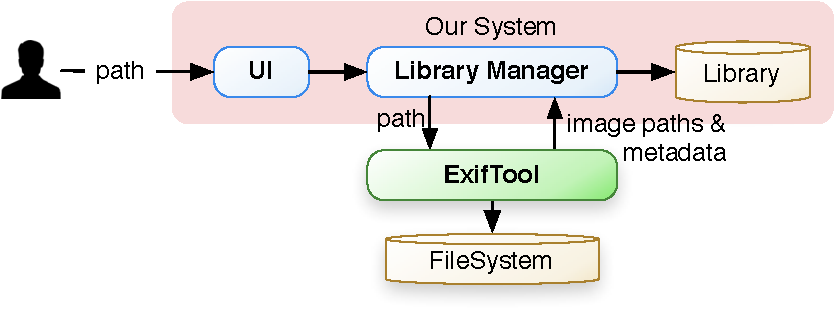
\includegraphics[scale=0.6]{Figures/import.pdf}
	\caption{Process in use by our system of importing a folder using ExifTool.}
	\label{fig:arch:import}
\end{figure}

Another option for importing metadata was to invoke EXIFTool as part of a \ac{FEP}. Although that could fix a couple of problems with the current  implementation, it doesn’t make the metadata as ubiquitous as needed. Most \acp{FEP} rely on some \ac{EXIF} plugins to work correctly and the current implementation doesn’t easily allow inter-\ac{FEP} data-sharing.

% subsubsection library_manager (end)




\subsubsection{Feature Extraction} % (fold)
\label{ssub:FeatureExtraction}

To arrange the images in the screen in different ways, they need to be classified. Some information is easy to optain and compare, like when the photograph was taken. Other information needs to be extracted, like the number of people in the photo or what are the most relevant colors in the image. \Fig{fe} is a short example of what feature extraction is all about.

\begin{figure}[ht]
	\centering
		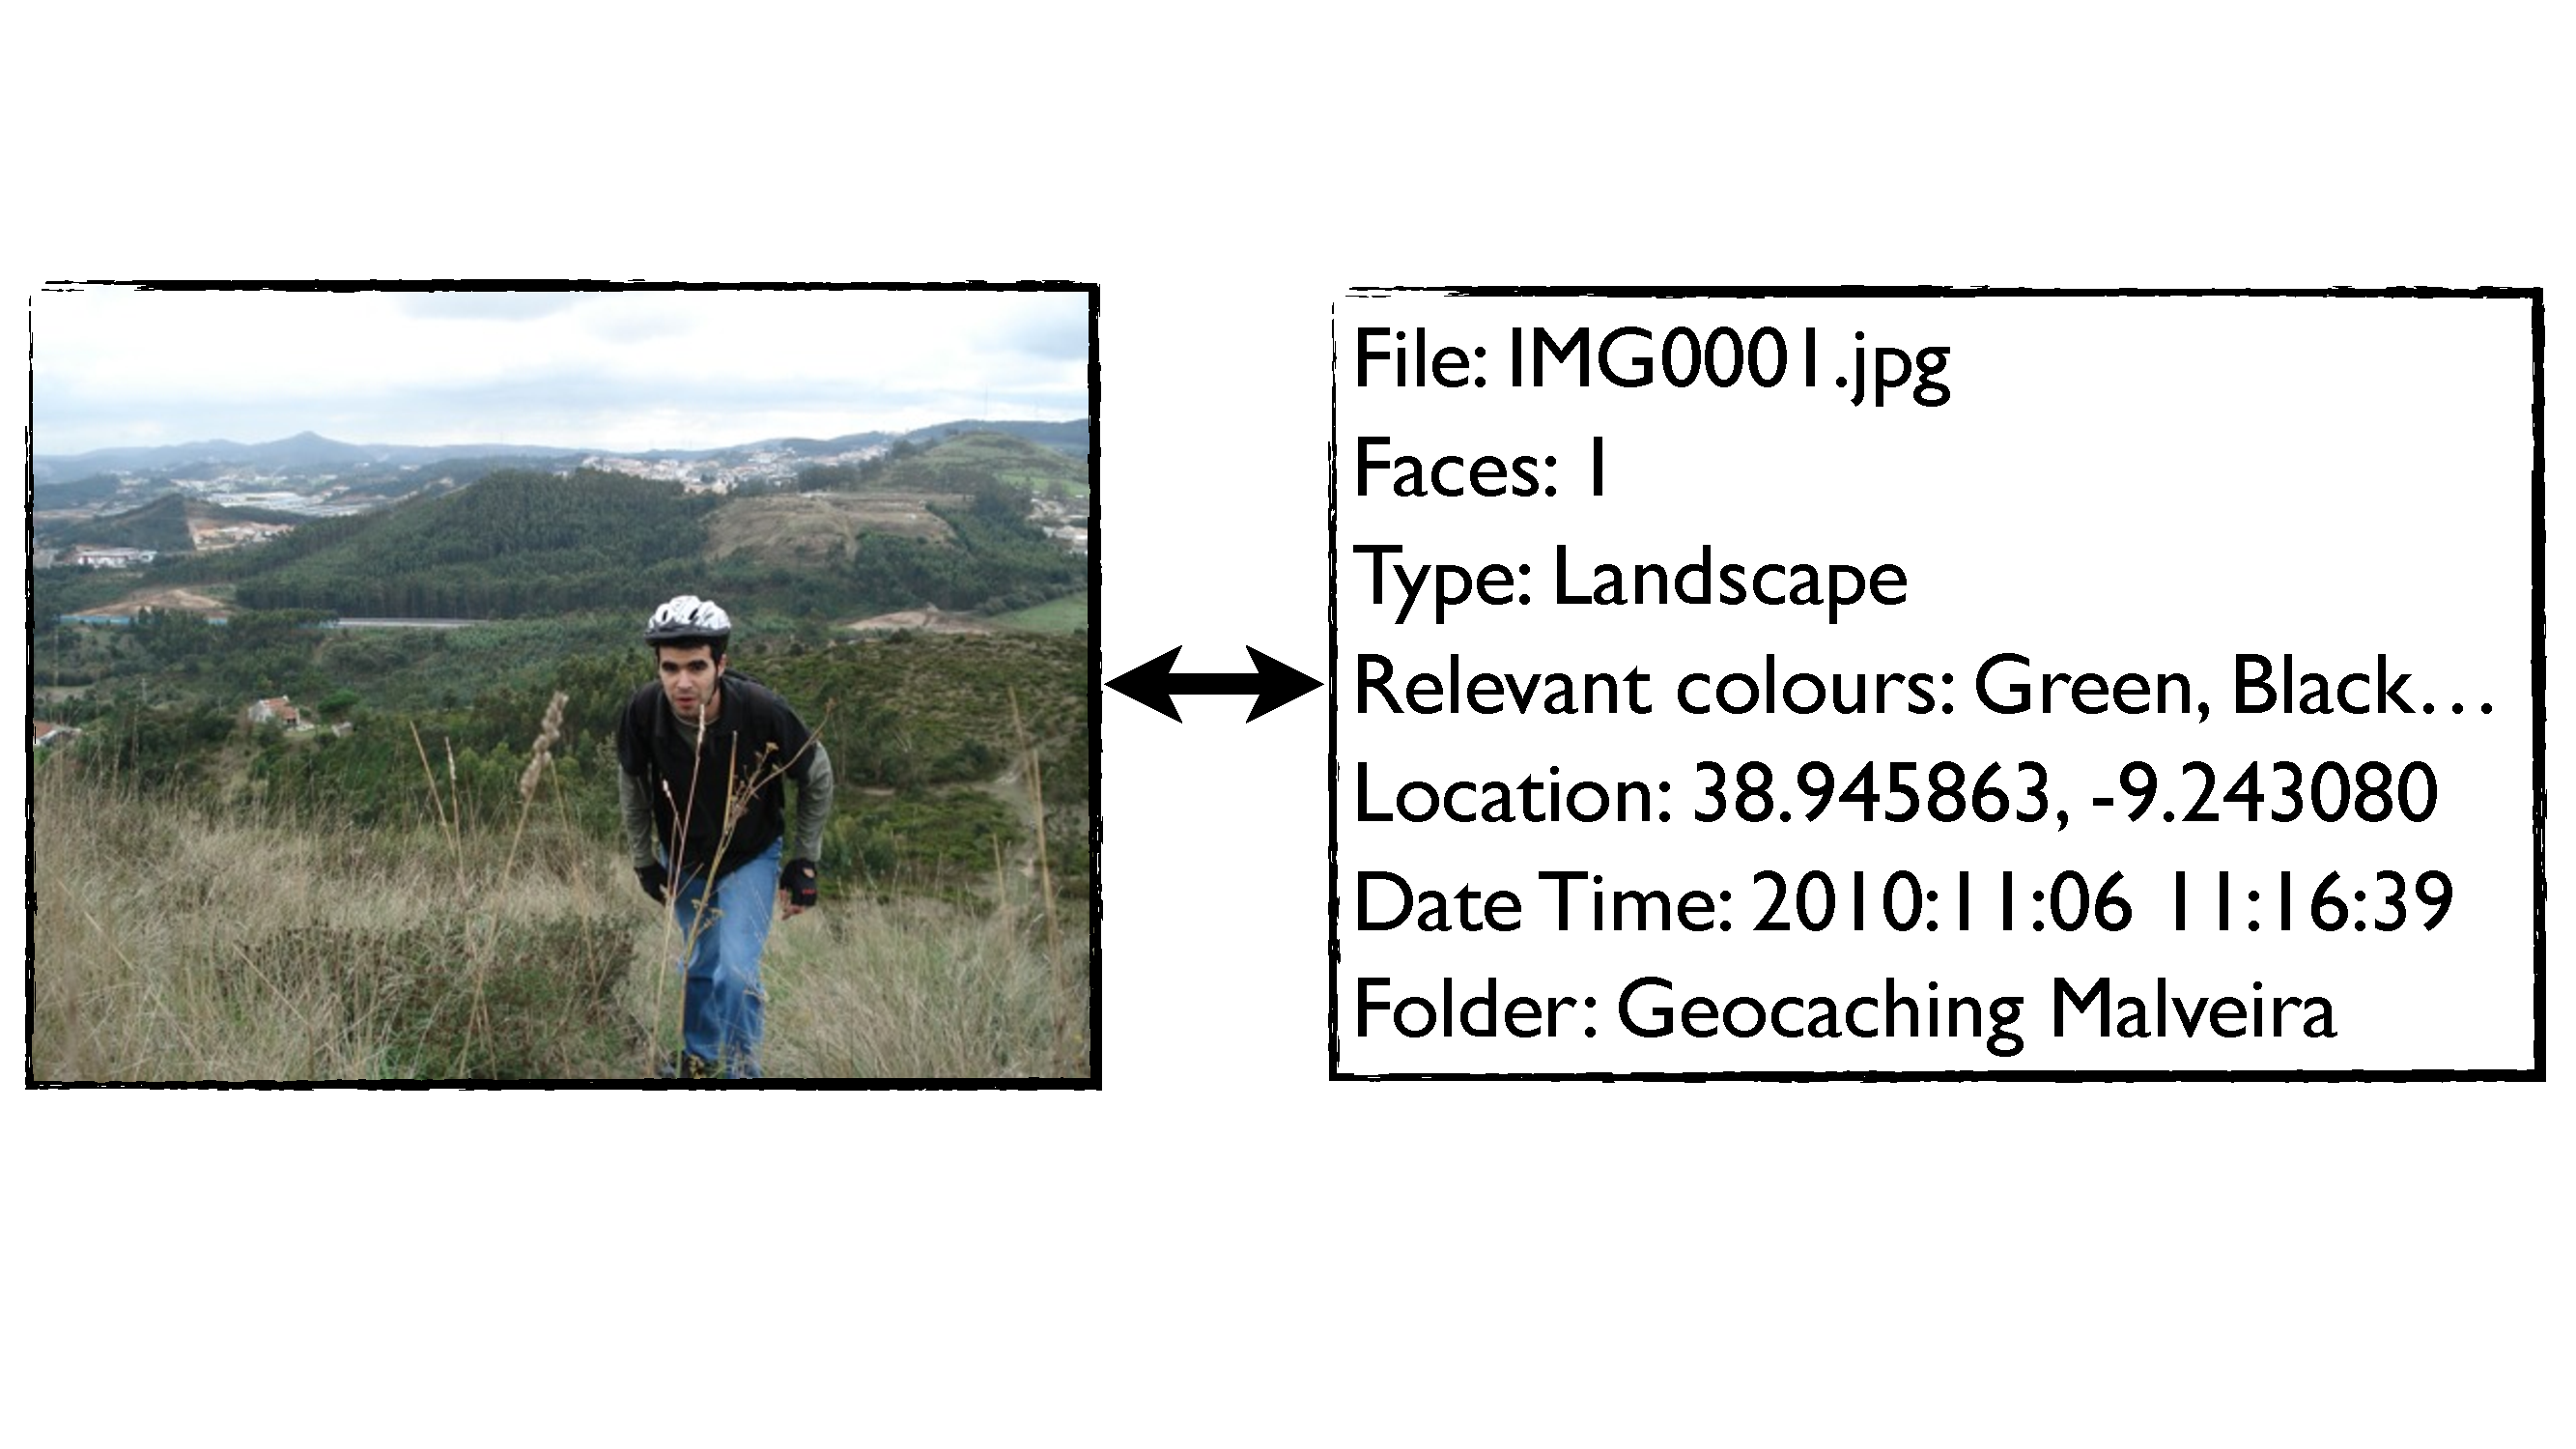
\includegraphics[width=0.72\columnwidth]{Figures/fe.pdf}
	\caption{Example of information extracted from an image.}
	\label{fig:fe}
\end{figure}

We had a few ideas for extracting features from images and, to be possible to add more along the way, we developed a plugin system to ease the creation of other plugins in the future.

Feature Extraction Plugins need to implement a common interface and are given the ability to process images and save the gathered data. They have freedom to access the image file or its \ac{EXIF} information and to structure the gathered data the way best suited for its purpose. They should, in the end, store the processed data in a specified way so it gets exported to the visualization. Existing plugins will be explained in section \ref{sub:plugins}.

% subsubsection Feature Extraction (end)




\subsubsection{Persistence} % (fold)
\label{ssub:Persistence}

Persistence of both library and plugin data are required so the system doesn't lose already gathered information. To ease the interaction with a database system, we created a database abstraction layer that hides the complexities of interacting with said system. It also allows us to change to another database system if we see the need for it. We chose Oracle's Berkeley DB\footnote{Berkeley DB is a high-performace, embeddable, key-value, file-based database available at \url{http://www.oracle.com/technetwork/database/berkeleydb}} for its speed in retrieving data.

With this layer we can hide some optimization complexities like lazy-saving and lazy-loading. We use lazy-saving to save data to disk by chunks instead of doing it on each small update, speeding up the update process. Lazy-loading is not yet implemented but it's essential with libraries with tens of thousands of images, where keeping a complete library in memory is not feasible.

% subsubsection database_abstraction_layer (end)

%subsection arch backend (end)












\subsection{Feature Extraction Plugins} % (fold)
\label{sub:plugins}

Currently, we have four feature extraction plugins:
\begin{itemize}
	\item Selection of useful image metadata
	\item Detection of image’s main color
	\item Face detection
	\item Generation of multi-scale imagery
\end{itemize}

We now proceed to the explanation of each one of this plugins. 

\subsubsection{Selection of useful image metadata}

This plugin acts as a filter for all the available \ac{EXIF} tags. It picks the most relevant, codes them in a defined way and appends them to the rest of the information to be exported for the visualization.

Information when the photo was captured, what device was used, the path where it resides or information about the location where the photo was taken are a good example of the most commonly relevant tags \todo{Ask users what other tags are relevant for them}. This set of extracted tags could be optionally set by the user.



\subsubsection{Detection of image’s main color}

Sometimes people don’t recall where or when a photo was taken, or where is it, but they vaguely remember, for instance, that the photo had some dominant color, for instance, the light blue of sky, the green of the grass or from a park, the dark blue of the sea, maybe some big red ball that someone was playing with. This information can be helpful when searching for a photo in a collection.

Color extraction from images has been a long standing problem \todo{insert a bunch of references for color detection}. One relevant work that we based this plugin is from Qiu et al\cite{Qiu:2007p1207} for exploring a method of image indexing that is fast and simple. On his work, images are sorted into ``bins'' according the their average color. This bins are divisions of color planes, indexed using binary trees allowing for very fast searches (\fig{qiu-color-regions}). For our plugin we used the open source library AForge.Imaging\footnote{AForge is a framework designed for developers and researchers in the fields of Computer Vision and Artificial Intelligence \url{http://www.aforgenet.com/framework/}} to obtain histograms for the images and compute their average color in RGB\footnote{Red, green and blue \url{http://en.wikipedia.org/wiki/RGB}} and HSL\footnote{Hue, saturation and luminance \url{http://en.wikipedia.org/wiki/HSL_and_HSV}} values. Both those values are then stored on the plugin-extracted data for each image.

\red{this probably shouldn’t be here}
This plugin demonstrates that color extraction is feasible and, with more time, a better method that does not average the colors but instead detects the most relevant ones could be implemented. \todo{references needed}

\todo{show of differences between having the image reduced or not. something I never tested :P}




\subsubsection{Face Detection} % (fold)
\label{ssub:face_detection}

The face detection plugin is based on the open-source OpenCV library\footnote{OpenCV (Open Source Computer Vision) is a library of programming functions for real time computer vision. Available at \url{http://opencv.willowgarage.com}} which processes every image file and detects existing faces (\fig{faces1}).
 
\begin{figure}[ht]
	\centering
		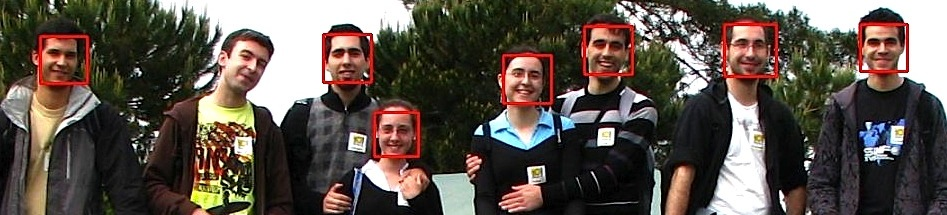
\includegraphics[width=\columnwidth]{Figures/faces1.jpg}
	\caption{Example of the OpenCV library detecting faces on a common photo.}
	\label{fig:faces1}
\end{figure}

No face recognition software is perfect. Usually if the software can detect every face, it will probably detect some other things in images that aren't faces (false positives). If it’s successful in only detecting faces, it will probably miss some other faces that aren't ideally positioned (false negatives). OpenCV is included in the latter, only detecting faces but also missing some that are tilted (like in \fig{faces1}) or turned on the side.


This process is quite computationally expensive and therefore we resize all the images down to a more acceptable size, making the process more than five times faster.

We tested 29 images, from six different cameras, ranging from one to ten megapixels, and containing up to thirteen faces. The test consisted in running face detection on each image, in its original size and in various resolutions from 2000 to 200 pixels on its longer side, comparing the number of faces recognised and the time needed to process them. The results can be seen in \fig{fdres}.

\begin{figure}[ht]
	\centering
		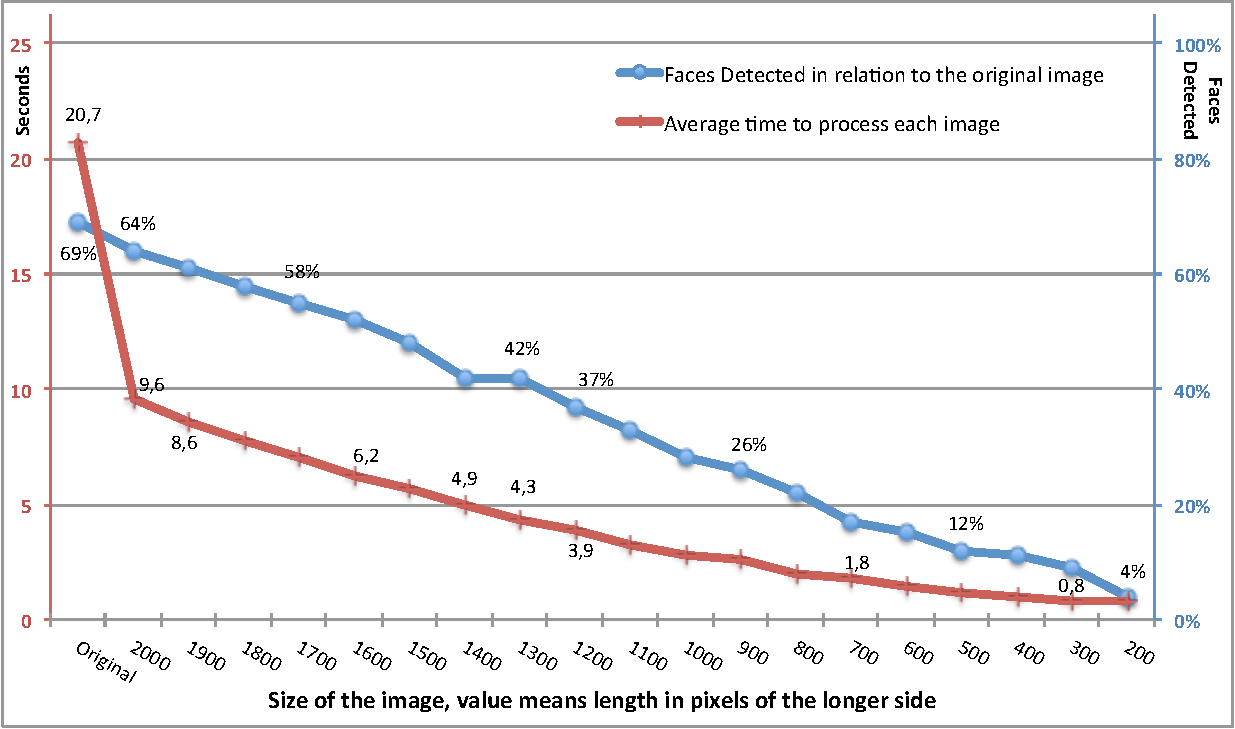
\includegraphics[width=\columnwidth]{Figures/graph2.pdf}
	\caption{Results of the face detection test. 100\% of faces is the actual faces present in the test images.}
	\label{fig:fdres}
\end{figure}

The purpose of this test is to identify how much can we reduce the images while maintaining a high recognition rate, we are comparing the recognition results of the downscaled versions to the original size and analyze the speedups and failures in recognition. We do include the number of faces actually present in the photos for comparison, corresponding to the 100\% value in \fig{fdres}.

We can see that by only reducing the images to 2000 pixels on the longer side, the processing time fell to less than half (20.7 to 9.6) without much loss in recognition (69\% to 64\%). The 1300 pixels was the chosen value for being the last with more than 40\% recognition rate (60\% of the full size image) and being 4.8 times faster\footnote{4.3 seconds per image versus 20.7; one hour and 10 minutes per thousand images versus almost six hours} than using the original image. In the future, with more tests, we can fine tune the resizing algorithm to get better results.



\hide{ver que caras falham primeiro para perceber o que aconteceu. As caras que se perdem são relevantes?}
% subsubsection face_detection (end)


\subsubsection{Generation of multi-scale imagery}

This plugin generates all the data files needed for the visualization to work. As referred previously, the visualization relies on the DeepZoom technology and it needs to process the images before they can be displayed. This plugin does exactly that.


Using a library from Microsoft, the plugin generates, for each image, a metadata file and a set of image files representing the original one at multiple scales, from a single pixel to a large, detailed image.

After passing through all images, the collection as a whole is subject of additional computation, this time generating imagery for all images as a single set and a metadata file that agglomerates all image sets used. This metadata file for the collection (called collection.xml) is then altered by the plugin to attach to each image, the data previously generated by the other plugins.

% subsection plugins (end)
